%; whizzy chapter
% -initex iniptex -latex platex -format platex -bibtex jbibtex -fmt fmt
% 以上 whizzytex を使用する場合の設定。

%     Kansai Debian Meeting resources
%     Copyright (C) 2007 Takaya Yamashita
%     Thank you for Tokyo Debian Meeting resources

%     This program is free software; you can redistribute it and/or modify
%     it under the terms of the GNU General Public License as published by
%     the Free Software Foundation; either version 2 of the License, or
%     (at your option) any later version.

%     This program is distributed in the hope that it will be useful,
%     but WITHOUT ANY WARRANTY; without even the implied warranty of
%     MERCHANTABILITY or FITNESS FOR A PARTICULAR PURPOSE.  See the
%     GNU General Public License for more details.

%     You should have received a copy of the GNU General Public License
%     along with this program; if not, write to the Free Software
%     Foundation, Inc., 51 Franklin St, Fifth Floor, Boston, MA  02110-1301 USA

%  preview (shell-command (concat "evince " (replace-regexp-in-string "tex$" "pdf"(buffer-file-name)) "&"))
% 画像ファイルを処理するためにはebbを利用してboundingboxを作成。
%(shell-command "cd image200708; ebb *.png")

%%ここからヘッダ開始。

\documentclass[mingoth,a4paper]{jsarticle}
\usepackage{kansaimonthlyreport}
\usepackage[dvips]{xy}
\usepackage{ulem}

% 日付を定義する、毎月変わります。
\newcommand{\debmtgyear}{2014}
\newcommand{\debmtgdate}{26}
\newcommand{\debmtgmonth}{1}
\newcommand{\debmtgnumber}{80}

\def\fixme#1{{\color{red}{#1}}}

\begin{document}

\begin{titlepage}

% 毎月変更する部分、本文の末尾も修正することをわすれずに

 第\debmtgnumber{}回 関西 Debian 勉強会資料

\vspace{2cm}

\begin{center}
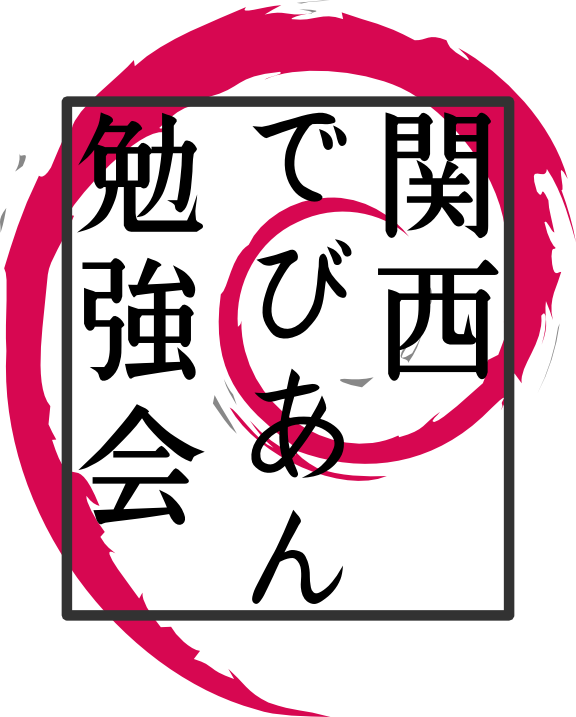
\includegraphics{image200802/kansaidebianlogo.png}
\end{center}

\begin{flushright}
\hfill{}関西 Debian 勉強会担当者 佐々木・倉敷・のがた・かわだ・八津尾 \\
\hfill{}\debmtgyear{}年\debmtgmonth{}月\debmtgdate{}日
\end{flushright}

\thispagestyle{empty}
\end{titlepage}

\dancersection{Introduction}{Debian JP}

\vspace{1em}

 関西Debian勉強会はDebian GNU/Linuxのさまざまなトピック
 (新しいパッケージ、Debian特有の機能の仕組、Debian界隈で起こった出来事、
 などなど)について話し合う会です。

 目的として次の三つを考えています。
 \begin{itemize}
  \item MLや掲示板ではなく、直接顔を合わせる事での情報交換の促進
  \item 定期的に集まれる場所
  \item 資料の作成
 \end{itemize}

 それでは、楽しい一時をお過ごしください。

\newpage

\begin{minipage}[b]{0.2\hsize}
 {\rotatebox{90}{\fontsize{80}{80}
{\gt 関西 Debian 勉強会}}}
\end{minipage}
\begin{minipage}[b]{0.8\hsize}
\hrule
\vspace{2mm}
\hrule
\setcounter{tocdepth}{1}
\tableofcontents
\vspace{2mm}
\hrule
\end{minipage}

\dancersection{最近のDebian関係のイベント報告}{Debian JP}

\subsection{第79回関西Debian勉強会}

79回目の関西Debian勉強会は12月22日(日)に、港区民センターで行なわれまし
た。

一年の振り返りと2014年の計画を行ないました。今年からは今までのセッショ
ン形式ではなく、ライトニングトークやもくもくの会を取り入れて行なってい
きます。

\subsection{第108回東京エリアDebian勉強会}

108回目の東京エリアDebian勉強会は1月18日(土)に株式会社スクウェア・エニッ
クス セミナールームで行なわれました。

野島さんによる「Debian Pure Blends」のセッションともくもくの会の形式で
行なわれました。東京も今年から形式を変えて開催されていきます。

\subsection{Debian Project}
\subsubsection{delegation}
今年度のDPLのLucasさんの活動にはdelegationという単語がよく目につきます。
ここ一月ほどのdebian-devel-announceのサブジェクトを追ってみただけでも
「Updating the Policy Editors delegation」
\footnote{\url{https://lists.debian.org/debian-devel-announce/2013/12/msg00004.html}}
「Updating the delegation for the Debian Keyring Maintainers (keyring-maint)」
\footnote{\url{https://lists.debian.org/debian-devel-announce/2013/12/msg00005.html}}
「Updating the delegation for the Debian Account Managers (DAM)」
\footnote{\url{https://lists.debian.org/debian-devel-announce/2013/12/msg00006.html}}
「Delegation for the Release Team」
\footnote{\url{https://lists.debian.org/debian-devel-announce/2013/12/msg00007.html}}
「Updating the Press Team delegation」
\footnote{\url{https://lists.debian.org/debian-devel-announce/2014/01/msg00001.html}}
「Updating the delegation for the Debian System Administrators (DSA)」
\footnote{\url{https://lists.debian.org/debian-devel-announce/2014/01/msg00002.html}}
と6通のメールが確認できます。

先月の活動報告
\footnote{\url{https://lists.debian.org/debian-devel-announce/2014/01/msg00005.html}}
にもあがっていますが、この活動のなかであいまいなところが確認されさらに
議論されており、組織として成熟してきているのかなと思います。

\subsubsection{Valve games for Debian Developers}
Debian Developerの特典としてLWNの購読権とGandi.netホスティング割引があ
りましたが、これにValveが提供するゲームへの無料サブスクリプションが追
加されそうです。
\footnote{\url{https://lists.debian.org/debian-devel-announce/2014/01/msg00006.html}}

これでDDになるモチベーションがまた一つ増えますね。

\subsubsection{ci.debian.net}
\url{ci.debian.net}という新しいサービスが稼動しています。unstableにある
DEP-8\footnote{\url{http://dep.debian.net/deps/dep8/}}
に対応したパッケージのテストを実施し、その結果を表示しています。まだ開発
中ですがそのうち公式アナウンスがでるでしょう。

\dancersection{事前課題}{Debian JP}

今回の課題は以下の通りです。
\begin{screen}
  \begin{enumerate}
  \item %
    Debian で、やろうとしてできていない上手くいってないこと、もしくは
    やろうとしていることを教えてください。

  \item %
    LT 歓迎です。何かお話したい方はタイトルを下さい。
  \end{enumerate}
\end{screen}

参加者の皆さんの解答は以下の通りです:

\begin{prework}{ 佐々木洋平 }
  \begin{enumerate}
  \item tDiary のパッケージングが上手くいってません。
  \item 「LT: jenkins + jenkins-debian-glue + freight で野良リポジトリ
    作った」です。
  \end{enumerate}
\end{prework}

\begin{prework}{ takata }
高田と申します。

最近の Debianの状況など、興味があるので飛び入り参加させて下さい。

以下、回答です。

(事前課題というよりも、ほとんど単なる質問になってしまいましたが...)


\begin{itemize}
\item 上手くいっていないこと: jessieで Redmineがうまく動作しない

最近はまっている未解決の問題なのですが、wheezyから jessieに upgradeした
マシンで Redmineが動かなくなってしまいました。

redmine関連のパッケージ、postgresql関連のパッケージをパージして、再イン
ストールしたりもしてみましたが、インストール時にエラーはとくに発生しな
いものの、アクセスすると ActiveRecord::ConnectionNotEstablishedのエラー
が発生し、postgresqlにうまく接続できていないようで、まったく何もブラウ
ザで表示されません。
\begin{commandline}
ii  redmine                  2.3.3-3.1  all  flexible project management web application
ii  redmine-pgsql            2.3.3-3.1  all  metapackage providing PostgreSQL dependencies for Redmine
ii  ruby                     1:1.9.3    all  Interpreter of object-oriented scripting language Ruby (default version)
ii  ruby-actionmailer-3.2    3.2.16-1   all  email composition, delivery, and receiving framework (part of Rails)
ii  ruby-actionpack-3.2      3.2.16-3   all  web-flow and rendering framework putting the VC in MVC (part of Rails)
ii  ruby-activemodel-3.2     3.2.16-1   all  toolkit for building modeling frameworks (part of Rails)
ii  ruby-activerecord-3.2    3.2.16-1   all  object-relational mapper framework (part of Rails)
ii  ruby-activeresource-3.2  3.2.16-1   all  REST modeling framework (part of Rails)
ii  ruby-activesupport-3.2   3.2.16-1   all  Support and utility classes used by the Rails 3.2 framework
ii  ruby-railties-3.2        3.2.16-2   all  MVC ruby based framework geared for web application development
\end{commandline}

ここで、ちょっと質問なのですが、\\
Debianの ruby関連の debパッケージとは別に、直接、gemパッケージをインス
トールすると競合して問題を起こすこともありそうですが、ruby関連のパッケー
ジは皆さんどのように使用されているのでしょう? 逆に、debパッケージは使
わずに gemパッケージだけを使っているとか...

\item その他の質問

Windows8ノート機に Debianをインストールする場合の推奨方法というのはある
でしょうか?

UEFIブートの場合、Windowsのブートマネージャから別パーティションにインス
トールした grubを起動してDebianをブートするのが無難なようにも思われるの
ですが、BCDの設定に関して、何か参考になる情報があれば教えていただけない
でしょうか。
\end{itemize}
\end{prework}

\begin{prework}{ 西山和広 }
  \begin{enumerate}
  \item squeeze のサポート終了が近くなってきたので、そろそろ wheezy に
    上げたいと思っていますが、まだ出来てません。
  \item さくらのVPSでIPv6設定
  \end{enumerate}
\end{prework}

\begin{prework}{ かわだてつたろう }
  \begin{enumerate}
  \item 
    \begin{itemize}
    \item イベントなどの会計整理。
    \item JP サイトのポリシー更新。
    \end{itemize}
  \end{enumerate}
\end{prework}

\begin{prework}{ 木下 }
  \begin{enumerate}
  \item 
    \begin{itemize}
    \item PANDABOARDへのGPUデバイスドライバのインストール。\\
       →NONフリーの為か、もしくは利用者が少ない為か情報が少ないように思います。
    \item 業務用システムOSとしての導入\\
       →CentOSを好まれてしまう(社内ですが・・・)。\\
       →クラウドサービス、データセンター等においてもDebianの選択肢が少ないような気がします。

    \end{itemize}
  \item 
     何かあればよいのですが・・・
  \end{enumerate}
\end{prework}

\begin{prework}{ 川江 }
  \begin{enumerate}
  \item kVMのVMでWWWサーバを立ち上げて、HTML5のサイトを作る予定。
  \item 特になし。
  \end{enumerate}
\end{prework}

\begin{prework}{ 榎真治 }
  \begin{enumerate}
  \item
    \begin{itemize}
    \item Becky!からsylpheedへのメールデータの移行と、ローカルでのimapサ
      ーバの設定(1つのメールアカウントでは成功したものの複数アカウント
        を扱う方法を調べ中)
    \item また、バージョンごとの動作の違いを調べたいので、LibreOfficeの
      TDFビルドを複数バージョン共存させる方法を探そうとしています。例え
      ば、4.1.4を入れると4.1.3は削除されます。
    \end{itemize}
  \end{enumerate}
\end{prework}

\begin{prework}{ yyatsuo }
  \begin{enumerate}
  \item 
    \begin{itemize}
    \item fcitx-skk のパッケージング
    \item kernel-handbookとDPNの翻訳
    \item RepRap on Debian 的なやつ
    \end{itemize}
  \item 時間があれば小ネタを用意します
  \end{enumerate}
\end{prework}

\begin{prework}{ lurdan }
  \begin{enumerate}
  \item Weblate の実験環境が壊れっぱなしなのでなんとかする
  \end{enumerate}
\end{prework}

\begin{prework}{ あかべ }
  \begin{itemize}
  \item apt-getするだけで統計機械翻訳システム一式を導入できるようにし
    たい。
    \begin{itemize}
    \item 翻訳・言語モデルの作成→フリーソフトウェアのドキュメントとか
      から取り出した対訳文を使って学習(だからフリー!)
    \item 利用例→フリーソフトウェアのドキュメントとかの翻訳作業を補助
    \end{itemize}
  \end{itemize}
\end{prework}

\begin{prework}{ 大北剛史 }
  \begin{enumerate}
  \item Kdeを使用しているが、resolutionをあげる方法がわかりません。
  \end{enumerate}
\end{prework}

\dancersection{ライトニングトーク}{}

\dancersection{今後の予定}{Debian JP}

\subsection{関西Debian勉強会}

次回、第81回関西Debian勉強会は2月23日(日)に福島区民センターで開催します。

\subsection{東京エリアDebian勉強会}
第109回東京エリアDebian勉強会は2月15日(土)に株式会社スクウェア・エニッ
クスの会議室でもくもくの会を主体に開催予定です。

%
% 冊子にするために、4の倍数にする必要がある。
% そのための調整
%% \dancersection{メモ}{}
%% \mbox{}\newpage
%% \mbox{}\newpage
%% \mbox{}\newpage

\printindex
%\cleartooddpage

 \begin{minipage}[b]{0.2\hsize}
  \rotatebox{90}{\fontsize{80}{80} {\gt 関西 Debian 勉強会} }
 \end{minipage}
 \begin{minipage}[b]{0.8\hsize}

 \vspace*{15cm}
 \rule{\hsize}{1mm}
 \vspace{2mm}
 
\includegraphics[width=2cm]{image200502/openlogo-nd.eps}
 \noindent \Large \bfseries{Debian 勉強会資料}\\ \\
 \noindent \normalfont \debmtgyear{}年\debmtgmonth{}月\debmtgdate{}日 \hspace{5mm}  初版第1刷発行\\
 \noindent \normalfont 関西 Debian 勉強会 (編集・印刷・発行)\\
 \rule{\hsize}{1mm}
 \end{minipage}

\end{document}
